\chapter{REVIEW OF RELATED LITERATURE}

We first present an introduction to the concepts in cryptography, starting from the definition of a cryptosystem up to homomorphic encryption schemes, along with some examples from the literature. Then, we present some concepts in image processing, a suitable application of cryptography, specifically the common image operations used. Finally, we present related work that attempts to apply image processing operations with homomorphic cryptosystems, as well as their advantages and limitations.

\section{Homomorphic Cryptosystems}
% [include mention of metrics by which they are compared]

In cryptography, a cryptosystem consists of an encryption function $\mathcal{E}$ and a decryption function $\mathcal{D}$, along with the plaintext space $\mathcal{P}$, ciphertext space $\mathcal{C}$ and the key space $\mathcal{K}$~\cite{bauer_cryptosystem_2005}. A \textit{plaintext} is text that can be commonly understood, while a \textit{ciphertext} results from encrypting the plaintext using an encryption key. The \textit{plaintext space} is the set of all possible plaintexts, the \textit{ciphertext space} is the set of all possible ciphertexts, while the \textit{keyspace} is the set of all possible keys.

There are two kinds of cryptosystems, \textit{symmetric} and \textit{asymmetric}. In symmetric-key cryptosystems, the same key is used for both encryption and decryption. As a consequence, symmetric-key cryptosystems must be implemented with a secure key exchange protocol, so that both the sender and receiver have access to the same key. Prominent examples of symmetric-key cryptosystems are the Data Encryption Standard (DES), and its replacement, the Advanced Encryption Standard (AES).

On the other hand, asymmetric-key (or public-key) cryptosystems use separate keys for encryption and decryption. The encryption key (also called the \textit{public key}) is shared to everybody, while the decryption key (also called the \textit{private key}) is kept secret. Since the public key and private keys are different, there is no need to agree upon secure key exchange protocols. Usually, the security of asymmetric-key cryptosystems relies on the intractability of certain computational problems, for example, the RSA cryptosystem depends on the difficulty of big integer factorization~\cite{rivest_method_1978}, while the ElGamal cryptosystem depends on the difficulty of the discrete logarithm problem~\cite{blakley_public_1985}.

Homomorphic cryptosystems are a special type of cryptosystem in which operations can be securely performed on encrypted data. Suppose that for a public-key cryptosystem, $\mathcal{E}_k \left(p \right)$ is the encryption function using the public key $k \in \mathcal{K}$, and $\mathcal{D}_l \left(c \right)$ be the decryption function using the private key $l$. A cryptosystem is said to be homomorphic if its encryption function is homomorphic, that is, if it satisfies the relation
\begin{equation}
    \mathcal{E}_k \left(p_1 \boxplus p_2\right) = \mathcal{E}_k \left(p_1\right) \boxdot \mathcal{E}_k \left(p_2\right)
\end{equation}
where $p_1, p_2 \in \mathcal{P}$ are the plaintexts, and $\boxplus$ and $\boxdot$ are operations in $\mathcal{P}$ and $\mathcal{C}$ respectively~\cite{fontaine_survey_2007}. Furthermore, a homomorphic cryptosystem also satisfies~\cite{li_elliptic_2012}
\begin{equation}
    p_1 \boxplus p_2 = \mathcal{D}_l \left( \mathcal{E}_k \left(p_1\right) \boxdot \mathcal{E}_k \left(p_2\right) \right).
\end{equation}
In other words, a homomorphic cryptosystem preserves the operations that can be done with the plaintext without requiring an intermediary step of decrypting the ciphertext beforehand. It is important to note that the operations $\boxplus$ and $\boxdot$ need not be the same. A simple operation in the plaintext space may require a computationally intensive operation in the ciphertext space.

Homomorphic cryptosystems are classified according to the plaintext and ciphertext operations, $\boxplus$ and $\boxdot$. If the plaintext operation $\boxplus$ is addition, the cryptosystem is said to be \textit{additively homomorphic}, and the cryptosystem is said to be \textit{multiplicatively homomorphic} if the plaintext operation $\boxplus$ is multiplication. Some examples of homomorphic cryptosystems include the Goldwasser--Micali cryptosystem~\cite{goldwasser_probabilistic_1984} and the Paillier cryptosystem~\cite{stern_public-key_1999}. Even some classic public-key cryptosystems are homomorphic, both RSA and ElGamal are multiplicatively homomorphic, while elliptic curve cryptosystems are additively homomorphic~\cite{li_elliptic_2012}. These cryptosystems, while relatively efficient, only support a limited set of operations on the encrypted data.

However, there exists \textit{fully homomorphic} cryptosystems, which are not limited to a fixed set of operations, but allow any arbitrary operations on the ciphertext. The first  fully homomorphic cryptosystem was presented by Gentry in 2009. Gentry's cryptosystem, which uses lattice-based cryptography, allows the computation of computation of arbitrary Boolean circuits on binary data~\cite{gentry_fully_2009, shortell_secure_2016}. New algorithms based on Gentry's initial ideas have since been made~\cite{ sen_homomorphic_2013}. One notable example is fully homomorphic cryptosystem by Smart and Vercauteren,~\cite{hutchison_fully_2010}, later improved by Gentry and Halevi ~\cite{hutchison_implementing_2011} which relies on cyclotomic number fields. In 2016, Dasgupta and Pal proposed a fully homomorphic cryptosystem based on polynomial rings~\cite{dasgupta_design_2016}. These two cryptosytems are examples of fully homomorphic cryptosystems which have significantly simpler encryption, decryption, addition and multiplication algorithms.

\section{Image Processing Operations}
The \textit{CryptoImg} library implemented several
We discuss two basic types of image processing operations, \textit{intensity transformations}, which map an intensity value to another, and \textit{spatial filters} which consider intensity values from regions of pixels to perform operations such as edge detection, image blurring and sharpening.

We represent a digital image $R$ as an $M \times N$ matrix of pixel intensity values, each value in the range $\left[0, L-1\right]$, for some positive integer $L$. We use $R(x,y)$ represents the entry at the $x$th row and $y$th column of a matrix $R$.

\subsection{Intensity Transformations}
An Intensity transformation on an image $R$ can be defined as a function $T$ which maps a pixel value $r$ to a new value $r^\prime$, which we can write as $r^\prime = T\left(r\right)$. This function is then applied to every pixel in $R$.

The \textit{CryptoImg} library implemented two types of linear intensity transformations: image negation and brightness control.
An image negation transformation is defined as:
\begin{equation}
    T\left(r\right) = L-1-r
\end{equation}
After applying image negation, the resulting image would be similar to a photographic negative~\cite{gonzalez_digital_2008}.

A brightness control transformation with parameter $v$ is defined as:
\begin{equation}
    T\left(r,v\right) = r+v
\end{equation}
The above transformations are linear in terms of the input $r$, and are thus simple to implement under a homomorphic cryptosystem.

In this study we extend the range of intensity transformations to non-linear transformations. Two common non-linear image transformations are the log transformation and power-law transformation~\cite{gonzalez_digital_2008}.

The log transformation is used to enhance dark pixels or increase the dark details of an image by mapping low intensity values to a wider range of values~\cite{gonzalez_digital_2008}. This has the general formula
\begin{equation}
    T\left(r\right) = c \log\left(1 + r\right)
\end{equation}
where $c$ is a constant and $r \ge 0$.

The power-law transformation is a family of transformations that have the form
\begin{equation}
    T\left(r\right) = c r^{\gamma}
\end{equation}
where $c>0$ and $\gamma > 0$.
A power-law transformation defined by the above equation can calibrate the operation of many image capture and output devices such as cameras, printers and displays in a process called \textit{gamma correction}. This ensures reproducibility and accuracy of images being displayed by digital output devices~\cite{gonzalez_digital_2008}.

To implement non-linear intensity transformations using addition and multiplication in a homomorphic system, it is necessary to approximate the logarithm and exponential functions, which may result in higher computational overhead. In our software library implementation, we investigate methods required to approximate the logarithm and functions.

\subsection{Spatial Filtering}
The \textit{CryptoImg} library also implemented \textit{spatial filters}. Spatial filters are operators which determine output pixels using information from neighboring input pixels. To apply a spatial filter to obtain a resulting image $R^\prime$, a convolution is performed between an $m \times n$ matrix $k$, called a kernel, and the original $M\times N$ image $R$.
A convolution between a kernel $k$ and image $R$ which yields a resulting image $R^\prime$, denoted as $R^\prime = k \ast R$, is defined by
\begin{align} \label{eq:spatialfilter}
	R^\prime(x,y) = \sum_{s=1}^m{\sum_{t=1}^n{k(s,t)R(x+s,y+t)}}, \text{ for all } 0\leq x \leq M, 0 \leq y \leq N,
\end{align}

\begin{figure*}[!ht]
    \centering
    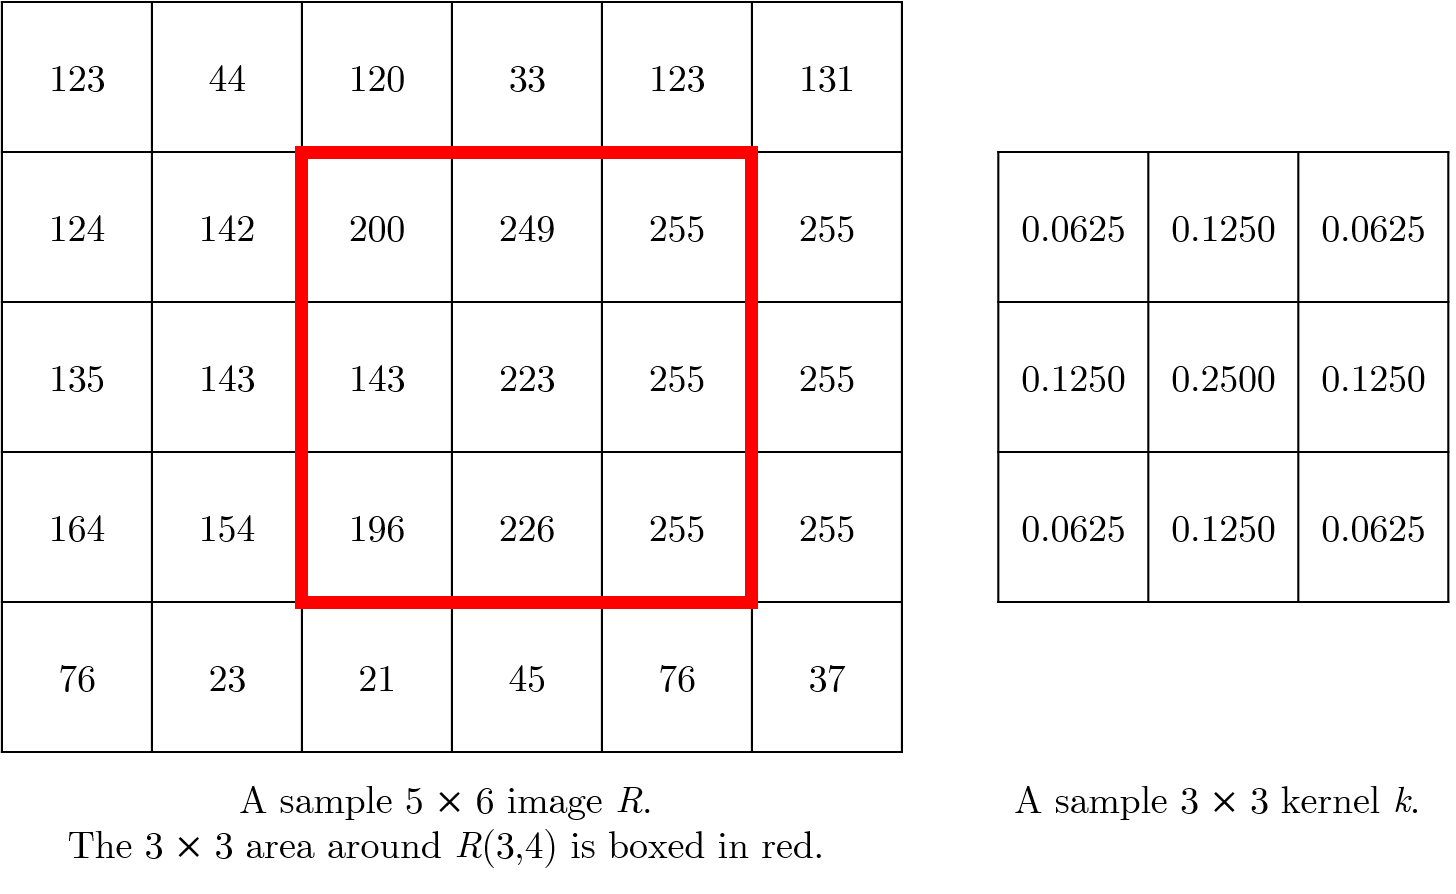
\includegraphics[width=\textwidth,\keepaspectratio]{Figures/SpatialFilter.png}
    \caption{A sample image $R$ and sample kernel $k$.}
    \label{fig:spatialfilter}
\end{figure*}
For example, using the image and $3 \times 3$ kernel given in Figure \ref{fig:spatialfilter}, we can calculate the value in the third row and fourth column of the resulting image $R^\prime$ by adding the products of entries in $k$ with the corresponding entries in $R$, found in an $3 \times 3$ region around $R(3,4)$.
\begin{align*}
	R^\prime(3,4) &= \sum_{s=1}^m{\sum_{t=1}^n{k(s,t)R(3+s,4+t)}}\\
	&= (0.0625\times 200) + (0.1250\times 249) + (0.0625\times 255) \\
	&+ (0.1250\times 143) + (0.2500\times 223) + (0.1250\times 255) \\
	&+ (0.0625\times 196) + (0.1250\times 236) + (0.0625\times 255)\\
	&= 223.
\end{align*}
Since spatial filters take values from a contiguous region of pixels, this presents a difficulty in homomorphic cryptosytems: in order for spatial filters to be performed, the location of each pixel relative to neighboring pixels has to be preserved. This was performed in the implementation of spatial filters in the \textit{CryptoImg} library~\cite{ziad_cryptoimg:_2016}. We wish to implement spatial filters using a similar approach, and assess how preserving spatial correlation between pixels can impact the security of the encrypted image.

\subsection{Common Spatial Filtering Kernels}
Edge detection is used to find and determine the boundaries in an image, commonly used in applications such as image segmentation and feature extraction. This works by detecting so-called \textit{edges}, areas that have abrupt changes in intensity.
One common method of performing edge detection is the Sobel operator, which uses two spatial filters to approximate the gradient of an image. Given an image $R$, and the kernels
\begin{equation}
    g_x =
    \begin{bmatrix}
        -1 & 0 & 1 \\
        -2 & 0 & 2 \\
        -1 & 0 & 1
    \end{bmatrix}
    \qquad\text{and}\qquad
    g_y =
    \begin{bmatrix}
        1 & 2 & 1 \\
        0 & 0 & 0 \\
        -1 & -2 & -1
    \end{bmatrix},
\end{equation}
$g_x \ast R$ yields the horizontal component of the gradient, while $g_y \ast R$ yields the vertical component of the gradient.

There are also spatial filters that perform image smoothing (such as Gaussian blur and box blur, which use the kernels $b_g$ and $b$ respectively in Equation~\ref{eqn:smooth-filters}) and image sharpening~\cite{gonzalez_digital_2008}.
\begin{equation}
    \label{eqn:smooth-filters}
    b_g = \frac{1}{16}
    \begin{bmatrix}
        1 & 2 & 1 \\
        2 & 4 & 2 \\
        1 & 2 & 1
    \end{bmatrix}
    \qquad
    b = \frac{1}{9}
    \begin{bmatrix}
        1 & 1 & 1 \\
        1 & 1 & 1 \\
        1 & 1 & 1
    \end{bmatrix}
\end{equation}

%% TODO: specific list of kernels to use for this study


\section{Related Work and Previous Implementations}
% CryptoImg

% example of homomorphic encryption / image manipulation past work

% minor limitation: improvement on previous work, but not a direct comparison

% major limitation: does not discuss security: are modified images also secure?

There has been work done regarding the application of homomorphic cryptosystems in image processing. In particular, Ziad, et al. introduced a library called \textit{CryptoImg} that uses the homomorphic properties of the Paillier cryptosystem to apply image operations securely \cite{ziad_cryptoimg:_2016}. This shows that it is indeed possible to do various image operations in a homomorphic cryptosystem. Ziad, et al. also showed experimental results establishing the slow performance of image operations uner a homomorphic cryptosystem. For instance, while sharpening and applying a Sobel filter each take less than a second when applied to a $512\times 512$ plaintext image, when applied to an encrypted image, sharpening required at least 238.257 seconds, and applying the Sobel filter required at least 147.567 seconds \cite{ziad_cryptoimg:_2016}.

However, a major limitation of \textit{CryptoImg} is that it does not consider image security. Even though the authors have established that the Paillier cryptosystem itself cannot be broken \cite{ziad_cryptoimg:_2016}, we believe that a cryptanalysis of the encrypted images after they have been operated is necessary, since image operations may be considered additional information in a known plaintext attack.

Furthermore, Ziad, et al. only presented a visual comparison and evaluation to establish the quality of the recovered images. We believe that additional image quality benchmarks, such as those presented in \cite{ahmed_benchmark_2016, ahmad_efficiency_2012}, would allow for quantitative comparisons of image quality.

This study can be further improved by also considering the use of fully homomorphic cryptosystems such as the one presented by Dasgupta and Pal \cite{dasgupta_design_2016}, and the fully homomorphic cryptosystem introduced by Smart and Vercauteren \cite{hutchison_fully_2010} and improved by Gentry and Halevi  \cite{hutchison_implementing_2011}. These fully homomorphic cryptosytems have yet to be implemented for image processing operations.

% HElib
Another related work would be the implementation of a fully homomorphic encryption. Halevi and Shoup \cite{garay_algorithms_2014} introduced \textit{HElib}, a library that implements the Brakerski--Gentry--Vaikuntanathan (BGV) homomorphic cryptosystem. This library also makes use of various optimizations to speed up the homomorphic operations, due to homomorphic cryptosystems being slower than other cryptosystems \cite{sen_homomorphic_2013}.

\section{Summary}
We have seen how various image processing operations make use of a series of additions and multiplications. Because of this, it is possible to use a homomorphic cryptosystem in order to apply image operations directly on encrypted images, as demonstrated by the \textit{CryptoImg} library.

In particular, we aim to address the shortcomings of \textit{CryptoImg} by developing a library to test various homomorphic encryption schemes with the help of the \textit{HElib} library to be able to implement fully homomorphic encryption schemes efficiently. This helps us determine the practicality of using homomorphic cryptosystems in image processing, especially when dealing with more complex image operations.
